\chapter{Problem Formulation and Related Work}
\label{ch:problem-related-work}

\section{Problem Formulation}
\label{ch:problem-formulation}

In \acrshort{acr:dtp} it is common to make use of a (compact) probabilistic model of the environment.
However, devising an optimal model for a specific system or process can be a daunting and error-prone task, when considering the wide range of possibilities while wanting a compact and computation-cost efficient model.

\section{Learning Probabilistic Models from Execution Traces}
\label{sec:learning-state-spaces}

\textbf{Iterative Adjustment of Probabilities}:
\begin{itemize}
	\item Likelihood maximization for Markov Chains/MDPs, which generalizes to Baum-Welch for HMMs/POMDPs
	\item Bayesian Inference (see section 2.2.1)
	\item Gradient-Ascent
\end{itemize}

\begin{figure}[]
	\centering
	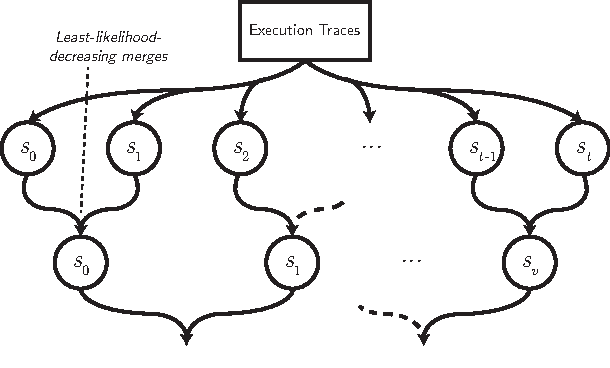
\includegraphics[width=0.8\textwidth]{model-merging-bfmm}
	\caption{State Merging}
	\label{fig:state-merging}
\end{figure}

\noindent \textbf{State Merging}:
\begin{itemize}
	\item Best-First Model Merging \cite{stolcke1994best}
	\item State Merging by Trajectory Clustering \cite{nikovski2000learning}
\end{itemize}

\noindent The other related work...

\section{Bayesian Reinforcement Learning}
\label{sec:bayesian-reinforcement-learning}

% https://people.eecs.berkeley.edu/~avivt/BRLS_journal.pdf
.....

% TODO;s
%% Fitting Markov Chains/MDPs:
	% Refer back to section 2.2.1:
	% - likelihood maximization
	% - Bayesian inference/optimization
%% Fitting HMMs/POMDPs:
	% ITERATIVE ADJUSTMENT OF PROBABILITIES:
	% - Baum-Welch Algorithm
	% - Gradient-Ascent in Likelihood
	% STATE MERGING
	% - Best-first
	% - Trajectory clustering
%% Reinforcement Learning: Online Model Learning

%% However, most of the previous works assume the state-space of the probabilistic model to be known.

%\section{Bayesian Reinforcement Learning}
%\label{sec:bayesian-reinforcement-learning}

% 

%
%\section{Overview}
%\label{sec:related-work-overview}
%
%% 